% Created 2025-08-18 Mon 23:56
% Intended LaTeX compiler: pdflatex
\documentclass[11pt,a4paper]{article}
\usepackage[utf8]{inputenc}
\usepackage[T1]{fontenc}
\usepackage{graphicx}
\usepackage{longtable}
\usepackage{wrapfig}
\usepackage{rotating}
\usepackage[normalem]{ulem}
\usepackage{amsmath}
\usepackage{amssymb}
\usepackage{capt-of}
\usepackage{hyperref}
\usepackage[margin=2.5cm]{geometry}
\usepackage{helvet}
\renewcommand{\familydefault}{\sfdefault}
\setlength{\parskip}{0.8em}
\setlength{\parindent}{0pt}
\author{Jorge Vargas}
\date{2025-08-18}
\title{Examen TA\textsubscript{2} – Aplicación \guillemotleft{}Comidita\guillemotright{}}
\hypersetup{
 pdfauthor={Jorge Vargas},
 pdftitle={Examen TA\textsubscript{2} – Aplicación \guillemotleft{}Comidita\guillemotright{}},
 pdfkeywords={},
 pdfsubject={},
 pdfcreator={Emacs 30.1 (Org mode 9.7.31)}, 
 pdflang={Spanish}}
\begin{document}

\maketitle
\section{Portada}
\label{sec:orgd60c0ec}
Este informe corresponde al examen TA\textsubscript{2} de la asignatura de Programación I.
Se presenta la aplicación \textbf{Comidita}, un sistema básico de restaurante desarrollado en Android con Kotlin y ConstraintLayout.
\section{Objetivos}
\label{sec:org4faa52f}
\begin{itemize}
\item Desarrollar una aplicación Android que permita simular el flujo de un pedido en un restaurante.
\item Aplicar conceptos de programación orientada a objetos mediante las clases \texttt{ItemMenu}, \texttt{ItemMesa} y \texttt{CuentaMesa}.
\item Usar \textbf{ConstraintLayout} para diseñar la interfaz de usuario.
\item Implementar la lógica de pedidos: agregar, quitar, calcular totales y propina.
\item Simular el envío de un pedido y reinicio de la aplicación.
\end{itemize}
\section{Desarrollo}
\label{sec:org7d87b0e}
\subsection{Repositorio github:}
\label{sec:orgf15e67e}
\url{https://github.com/afromankenobi/comidita}
\subsection{Clases principales}
\label{sec:orgd2a951e}
\begin{enumerate}
\item \texttt{ItemMenu}: representa un plato disponible (nombre y precio).
\item \texttt{ItemMesa}: representa un ítem pedido por la mesa (plato + cantidad).
\item \texttt{CuentaMesa}: gestiona el pedido total, sumando ítems, calculando subtotales, totales y propinas.
\end{enumerate}
\subsection{Actividad principal}
\label{sec:org248a57e}
\begin{itemize}
\item Se creó la actividad \texttt{MenuActivity}, que conecta los elementos de UI con la lógica de las clases.
\item Se usó \textbf{ConstraintLayout} para organizar botones, textos y controles.
\item Se implementaron botones para agregar y quitar ítems, un switch para la propina, y botones de control: \textbf{Nuevo pedido} y \textbf{Aceptar}.
\end{itemize}
\subsection{Lógica de flujo}
\label{sec:orge18bbc4}
\begin{itemize}
\item El usuario selecciona platos y cantidades.
\item La aplicación calcula subtotales, total y propina (10\%).
\item Al presionar \textbf{Aceptar}, se simula el envío del pedido (\textbf{ProgressBar}), y luego se confirma con un mensaje \textbf{Toast}.
\item Finalmente, la app reinicia la cuenta para tomar un nuevo pedido.
\end{itemize}
\subsection{Validación de negativos}
\label{sec:org01c7dd3}
Un detalle importante de la implementación es la validación para evitar cantidades negativas:
\begin{itemize}
\item Cuando la cantidad de un plato llega a 0, el botón de \textbf{restar} se deshabilita automáticamente.
\item Esto asegura que no se puedan ingresar valores inválidos y que la lógica de los cálculos (subtotal, total y propina) siempre sea consistente.
\item La validación se realiza tanto en el método \texttt{refrescarUI()} como en \texttt{setControlesEnabled()}, comprobando que la cantidad sea mayor a 0 antes de habilitar el botón de restar.
\end{itemize}
\subsection{Falta de imagenes}
\label{sec:orgc5eb0dc}
Me faltaron las imagenes, lo se. Perdón :(
\section{Capturas de Pantalla\hfill{}\textsc{ATTACH}}
\label{sec:org1fd3c39}
Aquí se insertarán las capturas de la aplicación en funcionamiento:

\begin{itemize}
\item Interfaz principal con los platos.
\end{itemize}

\begin{center}
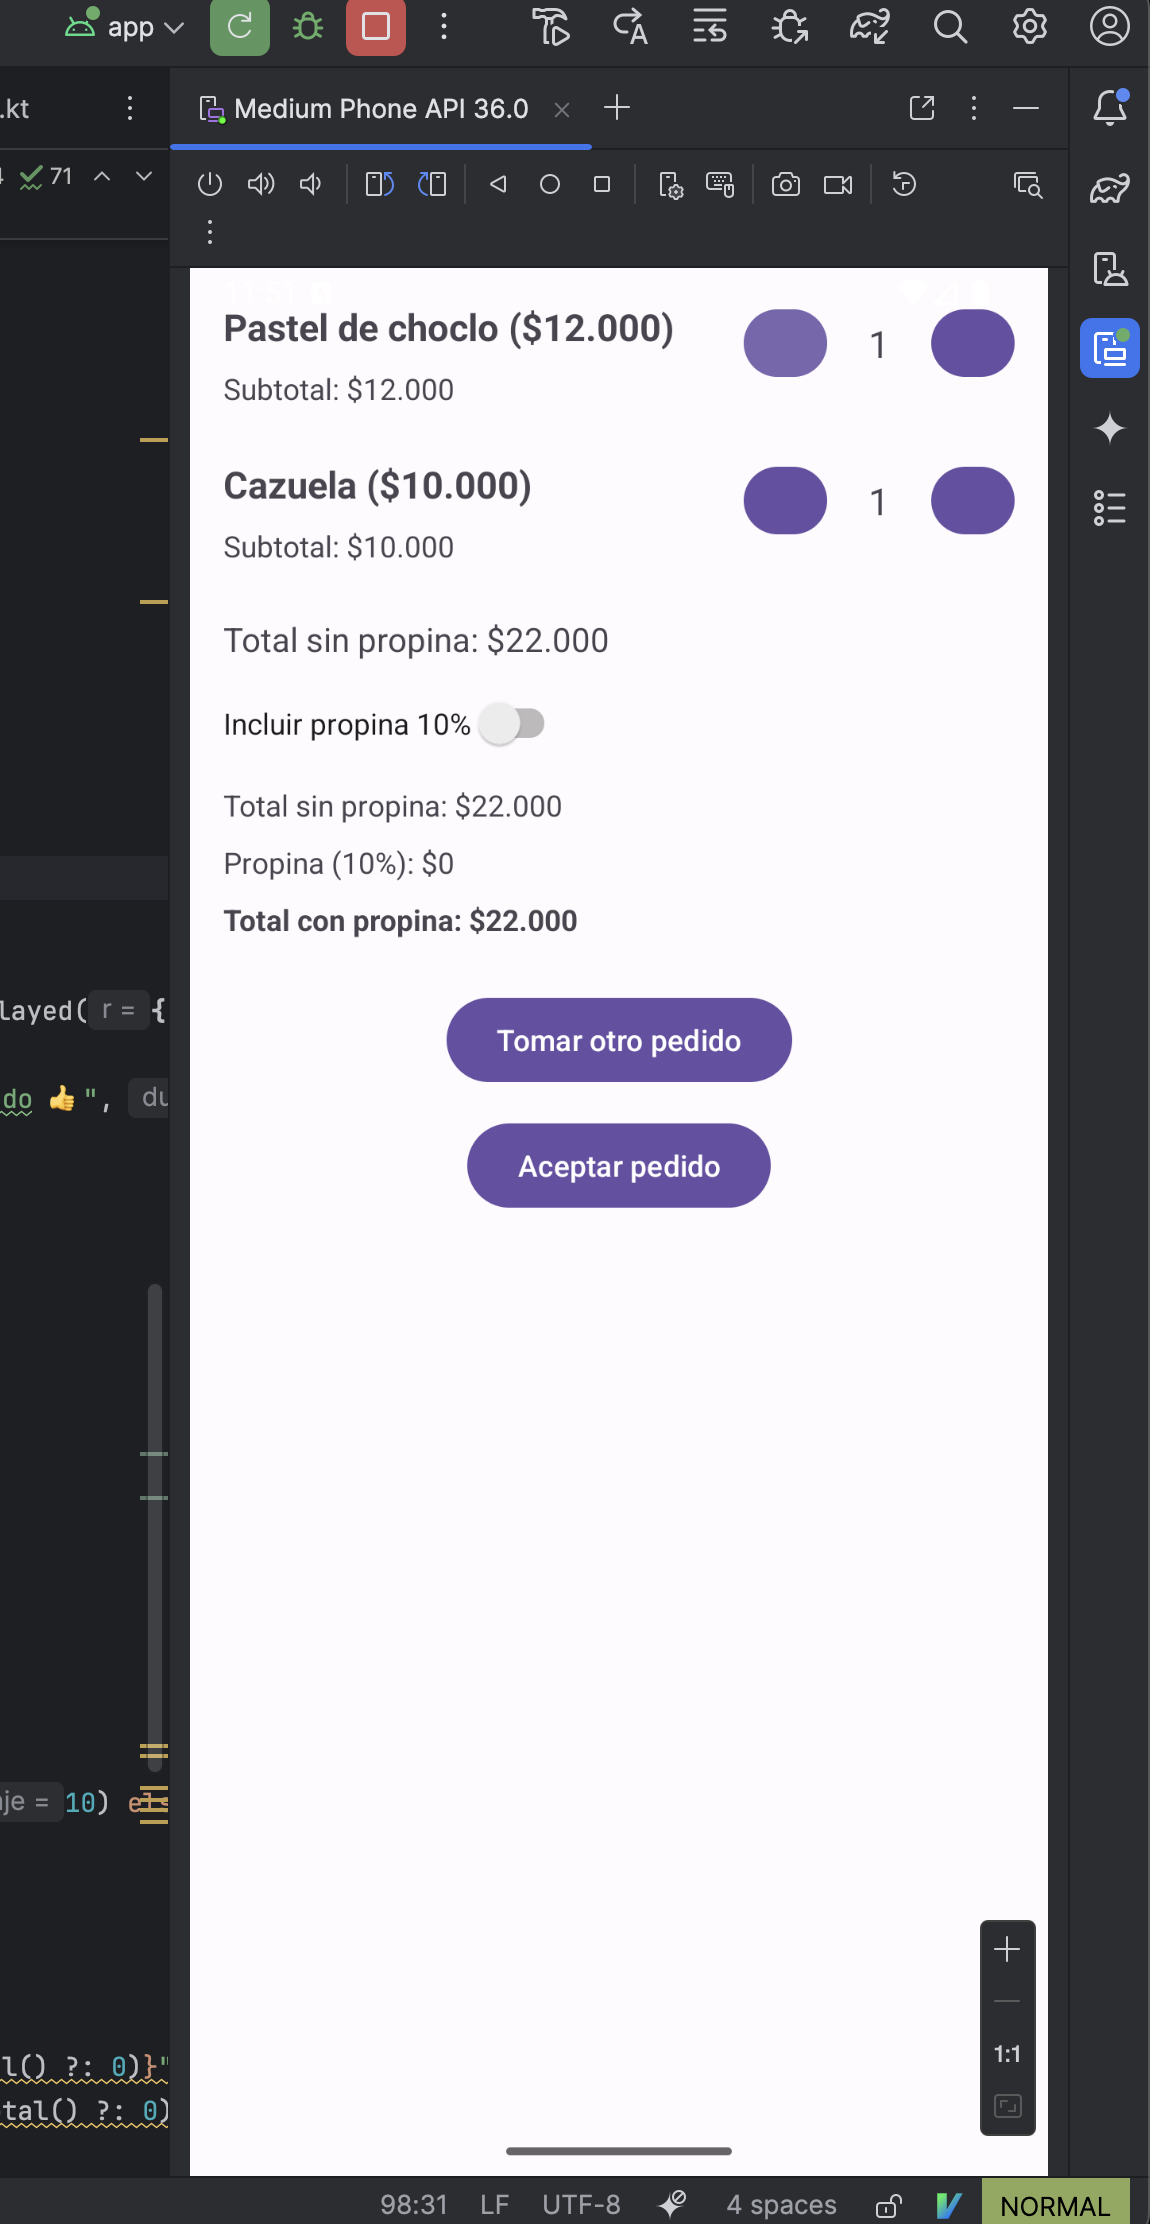
\includegraphics[width=.9\linewidth]{/Users/jvargas/orgfiles/.attach/5d/d718a0-a9d1-4b4f-80c2-dc33079d1fea/_20250818_235202screenshot.png}
\end{center}


\begin{itemize}
\item Simulación de envío del pedido (\textbf{ProgressBar}).
\begin{center}
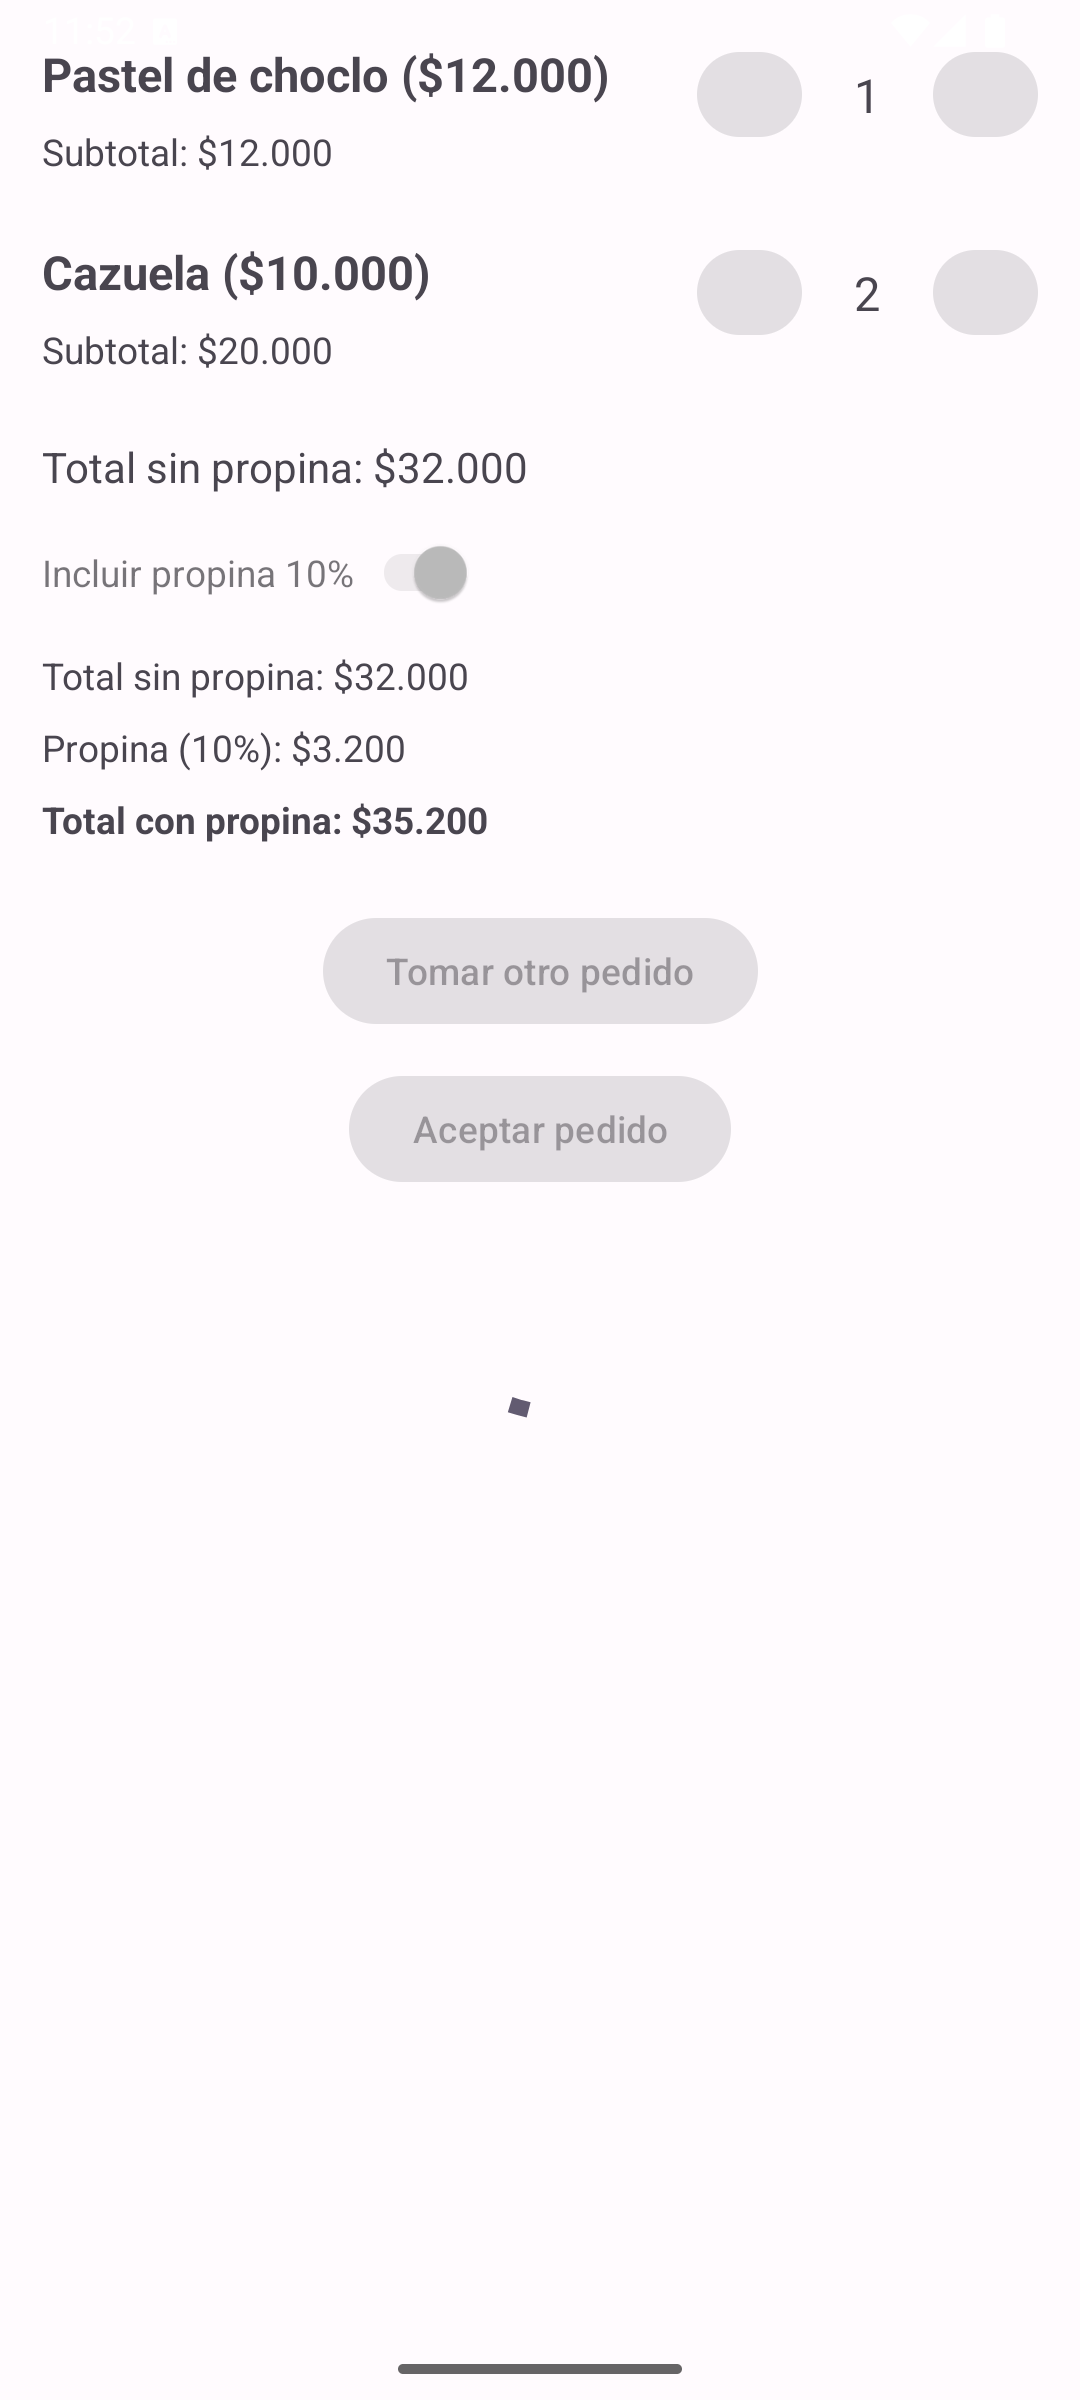
\includegraphics[width=.9\linewidth]{/Users/jvargas/orgfiles/.attach/5d/d718a0-a9d1-4b4f-80c2-dc33079d1fea/_20250818_235320screenshot.png}
\end{center}
\end{itemize}
\section{Conclusión}
\label{sec:org7433c29}

La aplicación cumple con los requerimientos de la prueba
\begin{itemize}
\item Implementa las clases necesarias
\item Integra la lógica con la interfaz en Android usando Kotlin y ConstraintLayout.
\item Valida adecuadamente que las cantidades de ítems no sean negativas.
\item Ofrece una experiencia básica pero completa de simulación de un pedido en un restaurante.
\item Permite reiniciar el proceso para múltiples pedidos.
\end{itemize}

\begin{quote}
Se logró aplicar los conceptos de POO y Android Studio, entregando un producto funcional, claro y extensible.
\end{quote}
\end{document}
